%!TEX program = lualatex

\documentclass[fleqn]{beamer}
\usetheme{metropolis}
\usepackage{graphicx}
\usepackage{comment}
\usepackage{color}
\usepackage[super]{nth}
\title{Image segmentation using SCIP}
\date{\today}
\author{Robert Schütz, Daniela Kilian}
\subtitle{Advanced practical SS 2017}

\usepackage{mathtools}

\newcommand{\superpixels}{\mathcal{S}}
\newcommand{\segments}{\mathcal{P}}

\usepackage{algpseudocode,algorithm}
\algnewcommand{\algorithmicgoto}{\textbf{goto}}%
\algnewcommand{\Goto}[1]{\algorithmicgoto~\ref{#1}}%

\usepackage{minted}

\begin{document}
	\maketitle
	
	\begin{frame}{Content}
		\setbeamertemplate{section in toc}[sections numbered]
		\tableofcontents
	\end{frame}

    \section{Problem definition}
	\begin{frame}{Task}
		\begin{figure}
            \begin{center}
               % \def\svgwidth{60mm}
                %\input{input.pdf_tex}
                
\includegraphics[width=60mm]{input}
                \caption{Input image}
            \end{center}
		\end{figure}
	\end{frame}

    \begin{frame}{Task}
        \begin{figure}
            \begin{center}
             %  \def\svgwidth{60mm}
               %\input{superpixels.pdf_tex}
               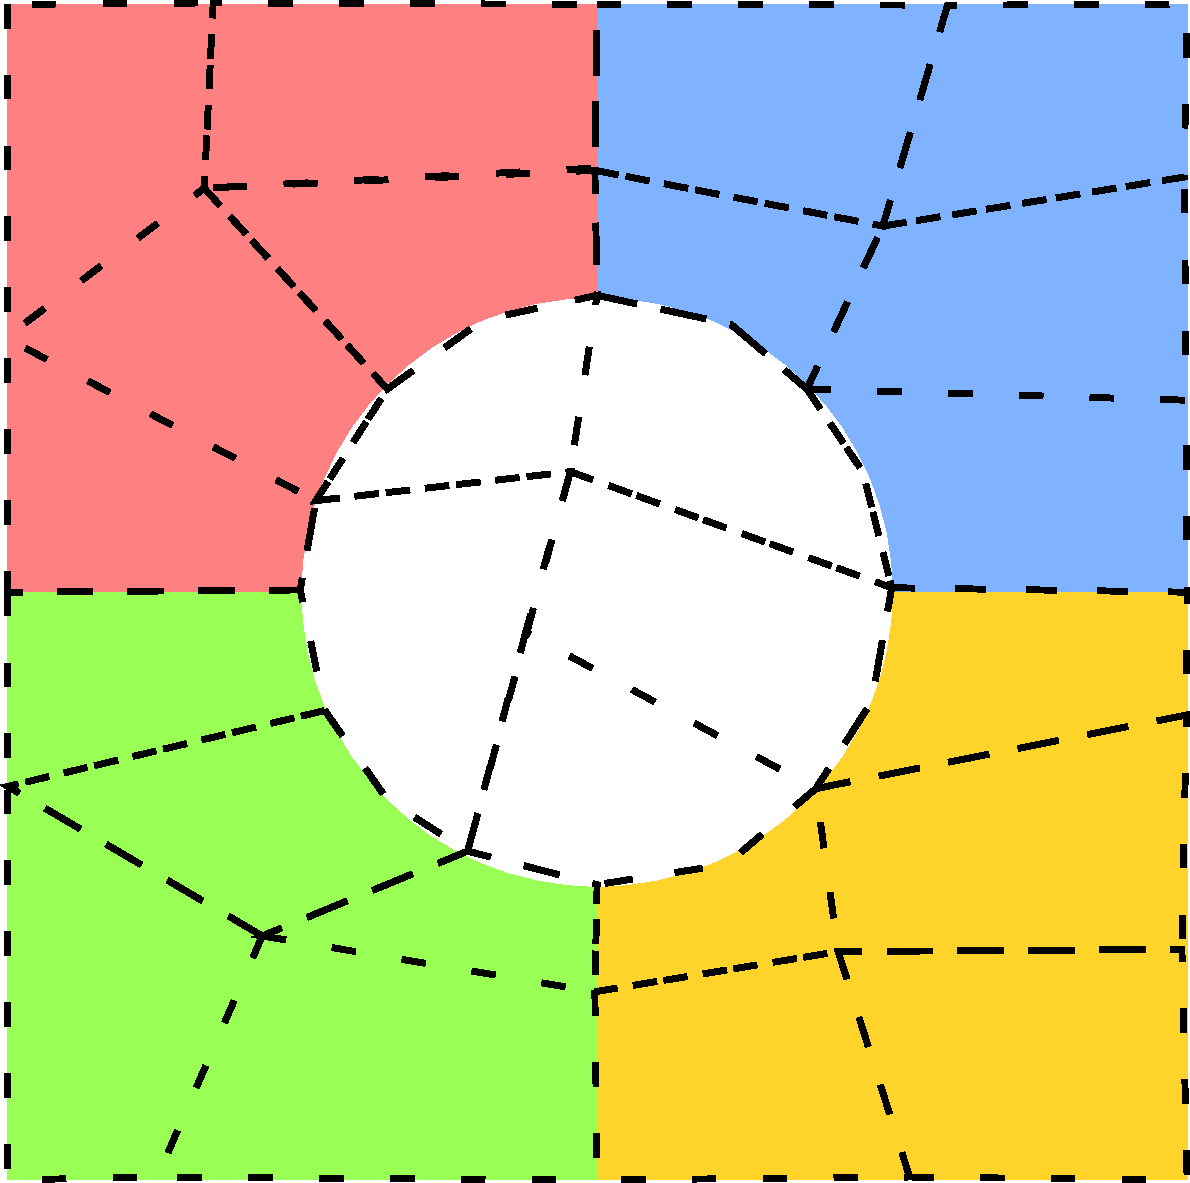
\includegraphics[width=60mm]{superpixels}
               \caption{Generated superpixels}
           \end{center}
        \end{figure}
    \end{frame}

    \begin{frame}{Task}
        \begin{figure}
            \begin{center}
                %\def\svgwidth{60mm}
                %\input{segments.pdf_tex}
                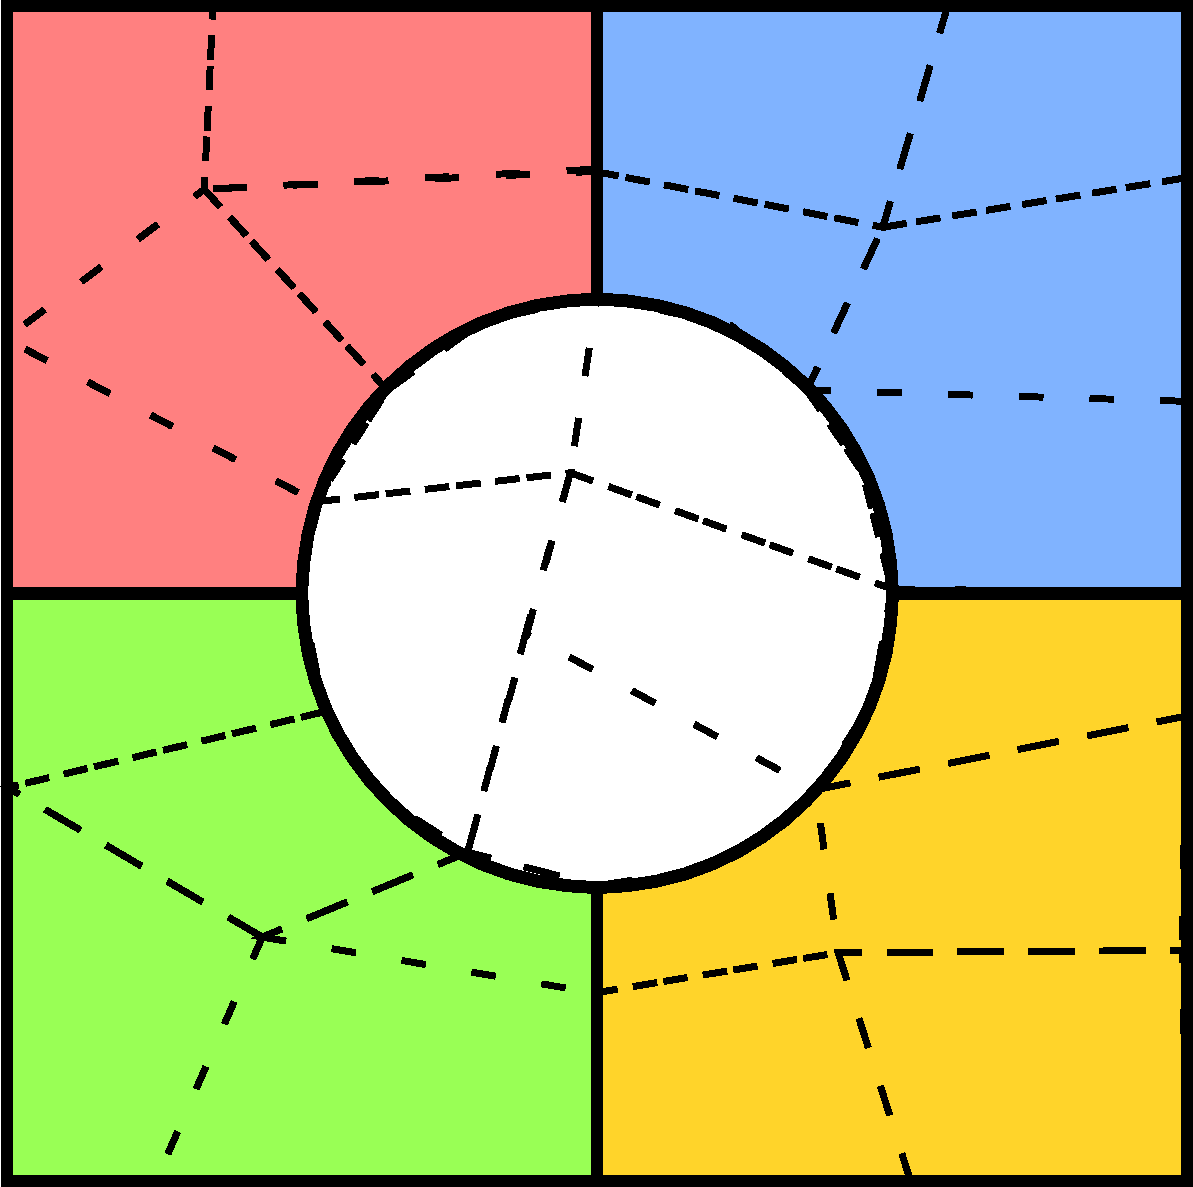
\includegraphics[width=60mm]{segments}
                \caption{Master nodes and segments}
            \end{center}
        \end{figure}
    \end{frame}	

    \begin{frame}{Master problem}
        Given data in the theoretical formulation of the master problem:
        \begin{itemize}
            \item $\superpixels$: set of superpixels
            \item $\segments$: set of segments %sagen: connected
            \item $y_s\geq0$: color of superpixel $s\in\superpixels$
            \item $T\subseteq\superpixels$: set of master nodes %number of segments to select = #T
            \item $k=|T|$: number of segments to cover the image with
            \item $r_P=\sum_{s\in P}|y_t-y_s|$: error of segment $P\in\segments$,
            where $t\in T$ is the single master node for which $t\in P$
        \end{itemize}
    \end{frame}
	
	\begin{frame}{Master problem}
		There is a binary variable $x_P$ for every segment $P\in\segments$.
        
		The problem reads as follows:
		\begin{align}
    		&\min\quad \sum_{P\in\mathcal{P}} r_P\cdot x_P\\
		    &\text{s.t.}\quad \smashoperator{\sum_{\{P\in\mathcal{P}:s\in P\}}} x_P = 1 \quad\forall s\in\superpixels \\
		    &\phantom{\text{s.t.}\quad} \sum_{P\in\mathcal{P}} x_P = k \\
		    &\phantom{\text{s.t.}\quad} x_P \in \{0,1\} \quad\forall P\in\segments
		\end{align}
	\end{frame}
	
	\begin{frame}{Dual problem}
		The dual variables are
		\begin{itemize}
			\item $\mu_s$ for all $s\in\superpixels$: corresponding to (2)
			\item $\lambda$: corresponding to (3)
		\end{itemize}
		
		The dual problem reads as follows:
		\begin{align}
		    &\max\quad \smashoperator{\sum_{s\in\superpixels}} \mu_s + k\cdot\lambda \\
		    &\text{s.t.}\quad \sum_{s\in P} \mu_s + \lambda \leq r_P \quad\forall P\in\mathcal{P} \\
		    &\phantom{\text{s.t.}\quad} \mu_s \text{ free} \quad\forall s\in\superpixels \\
		    &\phantom{\text{s.t.}\quad} \lambda \text{ free}
		\end{align}
	\end{frame}
	
	\begin{frame}{Pricing problem}
		There is a pricing problem for each master node $t\in T$,
		which generates a segment containing $t$.
		
		If $s\in\superpixels$ is in the new segment, then $x_s=1$.		
		 
		\begin{align}
    		&\min\quad \underbrace{\sum_{s\in\superpixels} x_s\cdot|y_t-y_s|}_{=r_{\{s\in\superpixels\ :\ x_s=1\}}} - \sum_{s\in\superpixels} x_s\cdot\mu_s \\
    		&\text{s.t.}\quad \text{connectivity constraint} \\
            &\phantom{\text{s.t.}\quad} x_t = 1 \\
            &\phantom{\text{s.t.}\quad} x_{t'} = 0 \quad\forall t'\in T\setminus\{t\} \\
	    	&\phantom{\text{s.t.}\quad} x_s \in\{0,1\} \quad\forall s\in\superpixels
		\end{align}
	\end{frame}
	
	\begin{frame}{Pricing problem}
		Constraint (6) of the dual problem is violated by the new segment if and only if
		\[\underbrace{\sum_{s\in\superpixels} x_s\cdot|y_t-y_s|}_{=r_{\{s\in\superpixels\ :\ x_s=1\}}} - \sum_{s\in\superpixels} x_s\cdot\mu_s < \lambda.\]
        
		Therefore, a new segment has to satisfy this inequality in order to be added to the master problem.
	\end{frame}
    
	\begin{frame}{Cutting planes}
		%We use a cutting planes approach to ensure connectivity of the new segments.
        %To this goal, we represent the superpixels as nodes in a graph.
        %Two superpixels are connected if they have adjacent pixels in the original image.
		
		%After solving the pricing problem,
		%we look at the subgraph of all $s\in\superpixels$ for which $x_s=1$.
		%If there is a component $C$ that is not connected to $t$,
		%we add the following cut for each $s\in C$:
        
		We look at the subgraph with vertices $\{s\in\superpixels:x_s=1\}$.
        If a component $C$ is not connected to $t$,
        we add a cut for each $s\in C$:
        \[\sum_{s'\in\delta(C)}x_{s'} \geq x_s\]
        
        \begin{figure}
            \centering
            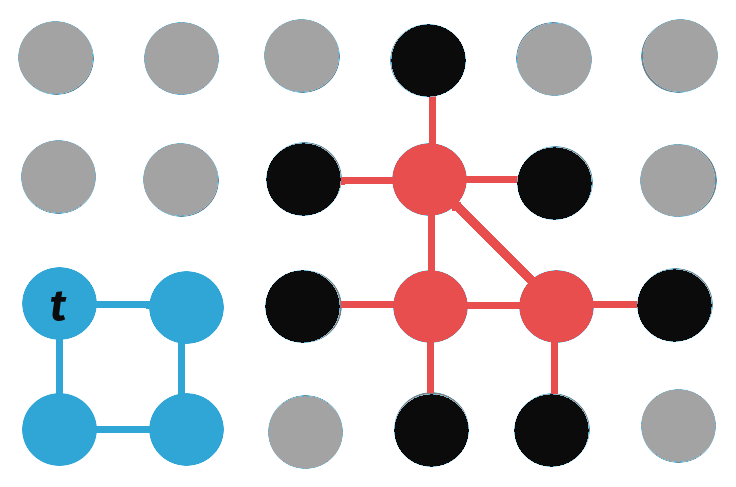
\includegraphics[scale=.2]{cuttingplanes.png}
            \caption{Violated connectivity constraint}
        \end{figure}
	\end{frame}
	
	\section{About SCIP}
	\begin{frame}{What is SCIP?}
		From \url{scip.zib.de}:
		\begin{quote}
			``SCIP is currently one of the fastest non-commercial solvers for mixed integer programming (MIP)
			and mixed integer nonlinear programming (MINLP).
			It is also a framework for constraint integer programming and branch-cut-and-price.''
		\end{quote}
	\end{frame}

    \begin{frame}{What is SCIP?}
        SCIP is developed at the Zuse Institute Berlin (ZIB).
        It is written in C, but can also be interfaced using
        \begin{itemize}
            \item C++
            \item Python
            \item Java
        \end{itemize}
    
        SCIP can use different LP solvers, e.g.
        \begin{itemize}
            \item SoPlex % also developed at ZIB
            \item CPLEX
        \end{itemize}
    \end{frame}

    \begin{frame}{What is SCIP?}
        \begin{figure}
            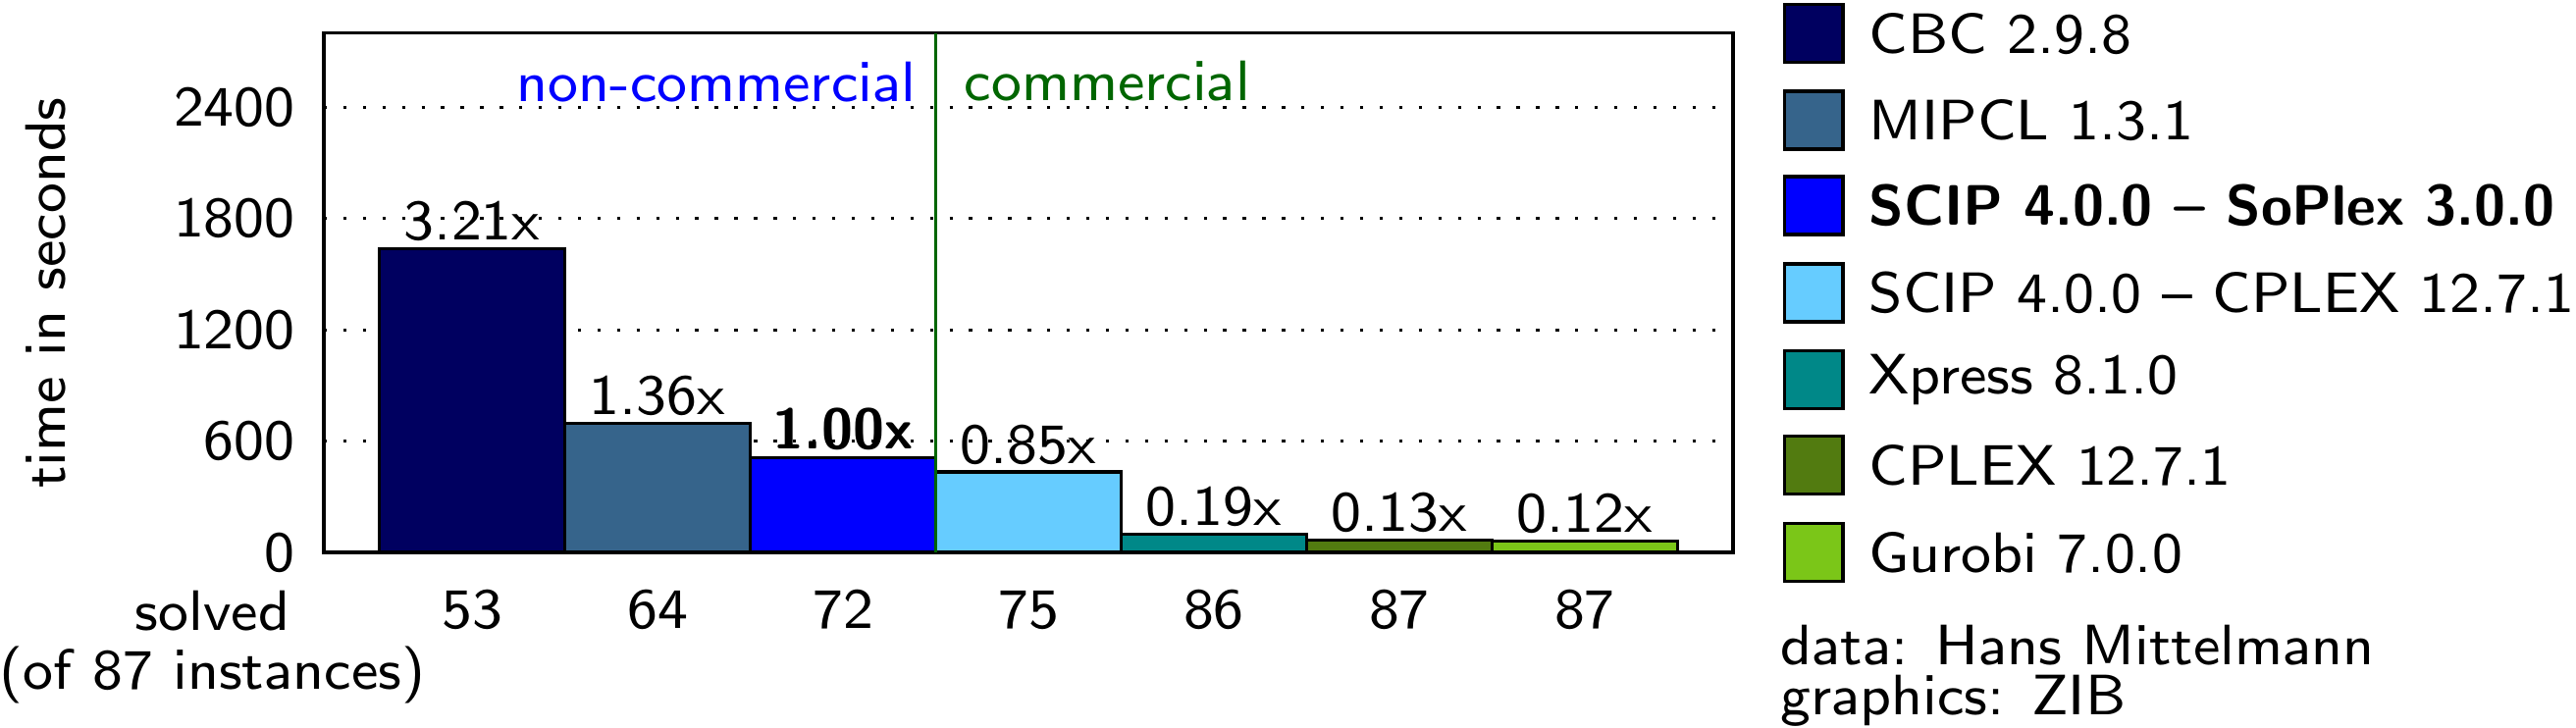
\includegraphics{comparison}
            \caption{MIP solver benchmark}
        \end{figure}
    \end{frame}

    \begin{frame}{Advantages}
        SCIP is non-commercial and open source.
    
        SCIP supports cutomizing
        \begin{itemize}
            \item Constraint handlers % d.h. eigene Arten von constraints und auch cutting planes
            \item Separators
            \item Variable pricers
            \item Branching rules
        \end{itemize}
        These use callbacks, so there is no need for a custom control loop.
        
        Also, SCIP can automatically do branching on variables declared as integral.
    \end{frame}
	
	\section{Implementation details}
    \begin{frame}{Programming Language}
        We are using C++.
        This makes it easy to interface with SCIP and add custom plugins.
        There are multiple SCIP examples written in C++, notably
        \begin{itemize}
            \item \textbf{VRP}, involving a custom pricer % vehicle routing problem
            \item \textbf{TSP}, involving a custom constraint handler % travelling salesman problem
        \end{itemize}
        We started off of these and implemented the desired functionality.
    \end{frame}

    \begin{frame}[fragile]{Reading the image}
        The image is first read from a PNG file using libpng and png++.
        Then, the image is segmented into superpixels using an algorithm called SLIC. %TODO reference SLIC
        
        \begin{minted}[fontsize=\tiny]{C++}
png::image<png::gray_pixel> pngimage(filename);
float* image = new float[pngimage.get_width() * pngimage.get_height()];
for (png::uint_32 x = 0; x < pngimage.get_width(); ++x)
{
  for (png::uint_32 y = 0; y < pngimage.get_height(); ++y)
  {
    image[x + y * pngimage.get_width()] = pngimage[y][x] / 255.0;
  }
}

segmentation = new vl_uint32[imagesize];
vl_slic_segment(segmentation, image, pngimage.get_width(), pngimage.get_height(), ...);
        \end{minted}
    \end{frame}
    
    \begin{frame}[fragile]{Creating the graph}
        To representing the graph of superpixels, we use the Boost Graph Library.
        
		\begin{minted}[fontsize=\tiny]{C++}
Graph g(superpixelcount);
for (auto p = vertices(g); p.first != p.second; ++p.first)
{
  g[*p.first].color = avgcolor[*p.first];
}	
// add edges
for (png::uint_32 x = 0; x < width; ++x)
{
  for (png::uint_32 y = 0; y < height; ++y)
  {
    auto current = x + y * width;
    auto right = x + 1 + y * width;
    auto below = x + (y + 1) * width;
    if (x + 1 < width
      && segmentation[current] != segmentation[right])
    {
      // add edge to the superpixel on the right
      auto edge = add_edge(segmentation[current], segmentation[right], g);
      auto weight = boost::get(boost::edge_weight, g, edge.first);
      boost::put(boost::edge_weight, g, edge.first, weight + 1);
    }
    ...
  }
}
		\end{minted}
	\end{frame}
	
	\begin{frame}[fragile]{Master problem definition}
        First, we need to create a SCIP instance.
        \begin{minted}[fontsize=\tiny]{C++}
SCIP* scip;
SCIP_CALL(SCIPcreate(&scip));
SCIP_CALL(SCIPcreateProb(scip, "master_problem", ...));
SCIP_CALL(SCIPsetObjsense(scip, SCIP_OBJSENSE_MINIMIZE));
        \end{minted}
        
        We start with initial segments which form a partitioning.
        \begin{minted}[fontsize=\tiny]{C++}
std::vector<SCIP_VAR*> vars;
for (auto segment : initial_segments)
{
  SCIP_VAR* var;
  // Set a very high objective value for the initial segments
  // so that they aren't selected in the final solution
  SCIP_CALL(SCIPcreateVar(scip, &var, "x_P", 0.0, 1.0, 10000, SCIP_VARTYPE_BINARY, ...));
  SCIP_CALL(SCIPaddVar(scip, var));
  vars.push_back(var);
}
        \end{minted}
    \end{frame}

    \begin{frame}[fragile]{Adding constraints}
        Finally, we add the partitioning constraints.
        \begin{minted}[fontsize=\tiny]{C++}
std::vector<SCIP_CONS*> partitioning_cons;
for (auto p = vertices(g); p.first != p.second; ++p.first)
{
  SCIP_CONS* cons1;
  SCIP_CALL(SCIPcreateConsLinear(scip, &cons1, "first", 0, NULL, NULL, 1.0, 1.0, ...));
  for (size_t i = 0; i != initial_segments.size(); ++i)
  {
    if (initial_segments[i].find(*p.first) != initial_segments[i].end())
    {
      SCIP_CALL(SCIPaddCoefLinear(scip, cons1, vars[i], 1.0));
    }
  }
  SCIP_CALL(SCIPaddCons(scip, cons1));
  partitioning_cons.push_back(cons1);
}

SCIP_CONS* num_segments_cons;
...
        \end{minted}
	\end{frame}

    \begin{frame}[fragile]{Pricer callback}
        \begin{minted}[fontsize=\tiny]{C++}
SCIP_DECL_PRICERREDCOST(scip_redcost)
{
  SCIP_Real lambda = SCIPgetDualsolLinear(scip, num_segments_cons);

  for (size_t i = 0; i < master_nodes.size(); ++i)
  {
    auto probdata = (PricerData*) SCIPgetObjProbData(scip_pricers[i]);
    for (auto s = vertices(g); s.first != s.second; ++s.first)
    {
      SCIP_Real mu_s = SCIPgetDualsolLinear(scip, partitioning_cons[*s.first]);
      SCIP_CALL(SCIPchgVarObj(scip_pricers[i], probdata->x[*s.first],
        -mu_s + std::abs(g[master_nodes[i]].color - g[*s.first].color)));
    }
    SCIP_CALL(SCIPsolve(scip_pricers[i]));
    SCIP_SOL* sol = SCIPgetBestSol(scip_pricers[i]);
    if (SCIPisDualfeasNegative(scip, SCIPgetSolOrigObj(scip_pricers[i], sol) - lambda))
    {
      SCIP_CALL(addSegmentVar(scip, scip_pricers[i], sol, master_nodes[i]));
    }
  }
  *result = SCIP_SUCCESS; // at least one improving variable was found,
                          // or it is ensured that no such variable exists
  return SCIP_OKAY;
}
        \end{minted}
    \end{frame}

    \begin{frame}[fragile]{Constraint handler callback}
        First, we create the subgraph of all superpixels in the new component. 
        \begin{minted}[fontsize=\tiny]{C++}
Graph& subgraph = g.create_subgraph();
std::vector<int> component(num_vertices(g));
for (auto p = vertices(g); p.first != p.second; ++p.first)
{
  if (SCIPisEQ(scip, SCIPgetSolVal(scip, sol, superpixel_vars[*p.first]), 1.0))
  {
    add_vertex(*p.first, subgraph);
  }
}
size_t num_components = connected_components(subgraph, &component[0]);
         \end{minted}
        
    \end{frame}

    \begin{frame}[fragile]{Constraint handler callback}
        \begin{minted}[fontsize=\tiny]{C++}
for (int i = 0; i < num_components; i++)
{
  if (i == component[master_node])
    continue;
    
  // all superpixels in the component
  std::vector<Graph::vertex_descriptor> superpixels = ...;
  // all superpixels surrounding the component
  std::vector<Graph::vertex_descriptor> surrounding = ...;
  
  for (auto s : superpixels)
  {
    // add a constraint/row to the problem
    SCIP_ROW* row;
    SCIP_CALL(SCIPcreateEmptyRowCons(scip, &row, conshdlr, "sepa_con",
      0.0, SCIPinfinity(scip), ...));

    // sum_{all superpixels s surrounding the component} x_s >= ...
    for (auto s_ : surrounding)
      SCIP_CALL(SCIPaddVarToRow(scip, row, superpixel_vars[s_], 1.0));

    // ... >= x_s
    SCIP_CALL(SCIPaddVarToRow(scip, row, superpixel_vars[s], -1.0));

    SCIP_CALL(SCIPflushRowExtensions(scip, row));
    SCIP_CALL(SCIPaddCut(scip, sol, row, ...));
  }
}
        \end{minted}
    \end{frame}

    \begin{frame}[fragile]{Solve master problem}
        \begin{minted}[fontsize=\tiny]{C++}
// include pricer 
ObjPricerLinFit* pricer_ptr = new SegmentPricer(scip, g, ...);
SCIP_CALL(SCIPincludeObjPricer(scip, pricer_ptr, true));

// activate pricer 
SCIP_CALL(SCIPactivatePricer(scip, SCIPfindPricer(scip, "pricer")));

// solve
SCIP_CALL(SCIPsolve(scip));
SCIP_SOL* sol = SCIPgetBestSol(scip);

// return selected segments
std::vector<std::vector<Graph::vertex_descriptor>> segments;
SCIP_VAR** variables = SCIPgetVars(scip);
for (int i = 0; i < SCIPgetNVars(scip); ++i)
{
  if (SCIPisEQ(scip, SCIPgetSolVal(scip, sol, variables[i]), 1.0))
  {
    auto vardata = (ObjVardataSegment*) SCIPgetObjVardata(scip, variables[i]);
    segments.push_back(vardata->getSuperpixels());
  }
}
        \end{minted}
    \end{frame}
        
	\section{Possible improvements}
    \begin{frame}{Pricing heuristic}
        To make the solving process faster,
        a heuristic to find segments with negative reduced costs ($rc$) should be added.
        
        \begin{algorithm}[H]
            \caption{Simple pricing heuristic}
            \begin{algorithmic}[1]
                \State $P\gets\{t\}$
                \State Let $s\in\delta(P)$ s.t. $rc(P\cup\{s\})$ is minimal. \label{nextnode}
                \If {$rc(P)\geq0$}
                    \State $P\gets P\cup\{s\}$
                    \State \Goto{nextnode}
                \ElsIf {$rc(P\cup\{s\}) < rc(P)$}
                    \State $P\gets P\cup\{s\}$
                    \State \Goto{nextnode}
                \Else
                    \State \Return $P$
                \EndIf
            \end{algorithmic}
        \end{algorithm}
    \end{frame}

    \begin{frame}{Branching rules}
        Ideally, one would develop branching rules specially for the master and pricing problem.     
        
        For example, branching on segments with minimal objective values could lead to good results.
        
        This is out of scope for this practical.
    \end{frame}
    
    \section{Demo}
\end{document}
